%%%%%%%%%%%%%%%
%
% $Autor: Wings $
% $Datum: 2020-01-29 07:55:27Z $
% $Pfad: komponenten/Bilderkennung/Produktspezifikation/IntelNCS2/Inhalt/Einleitung.tex $
% $Version: 1785 $
%
%
%%%%%%%%%%%%%%%


%todo citatzions in correct manner
\chapter{Einleitung}


{\tiny Quelle: \url{https://www.arduino.cc/pro/tutorials/portenta-h7}}


\chapter{Indroduction}


Arduino is an open-source electronics platform based on flexible, easy-to-use hardware and software. It provide us on board microcontroller and microprocessor kits for making digital and analogue devices. The microcontroller, oftenly called as tiny computer embed on the arduino board, normally in order to run these microcontroller we need some type of electronics e.g; diodes, resisters, capacitors, and transistors for making the voltage and current balancing. But the arduino team make a user friendly environment for getting rid of these electronics complication to run the hardware on software, just power the board as per the required voltage write the desired programm and upload it in a few seconds, it will bring everything on the board and  make us independent from any worry about the electronics complication. By the technological advancement in semiconductor and electronics  industry, the  control problems are now being solved by using these small size microcontroller instead of mechanical and electrical swithes. All Arduino boards have one thing in common which is a microcontroller, it is basically a really small computer, which help us to make a edge computing application.\cite{Arduino:2021b}

\section{Arduino Nano 33 BLE Sense}


Arduino Nano 33 BLE Sense is one type of arduino family board, which is come up with bluetooth capability for communication and set of sensors. This compact and reliable Nano board is built around the NINA B306 module for BLE and Bluetooth 5.0 communication; Bluetooth 5.0 is the latest version of the Bluetooth wireless communication standard. Use of microcontrollers has become inevitable in almost every field of engineering.  The Arduino Nano 33 BLE Sense module is based on Nordic nRF52480 processor that contains a powerful Cortex M4F and the board has a rich set of sensors that allow the creation of innovative and highly interactive designs. Its reduced power consumption, compared to other same size boards, together with the Nano form factor opens up a wide range of applications. The following figure ~\ref{Arduino Nano} shows a Arduino Nano 33 BLE Sense, shows how compact it is and small in size.

\begin{figure}[ht]
	\centering
	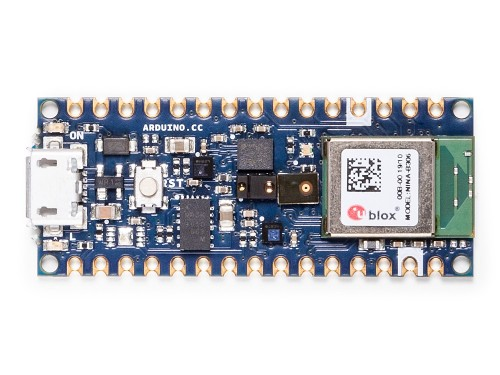
\includegraphics[width=0.45\linewidth]{Arduino/ArduinoNano33BLESense}
	\caption{Arduino Nano 33 BLE Sense} 
	\label{Arduino Nano}
\end{figure}

Due to the Bluetooth low energy (BLE) and set of sensors which are emded on it, this arduino board makes a perfect match for tiny Machine learning and IOT application. Bluetooth is used for communication between Arduino board and external devices. 

\section{On-Board Sensor Description}

Arduino Nano 33 BLE sense come up with the set of embed sensor on the board. The available embed sensors are commonly use for measuring both the analog and digital values around the sorrounding. Arduino Nano 33 BLE sense is very small (45x18)mm in size, which  makes it very usefull for Internet of things (IOT) and Artificial intelligence (AI) application as a embed device where space is the main constrained issue. It is low power consumption board and operate normally on 3.3 V, we can say that this small size low power consumption board can operate on small batteries even for many months. Due to on-board available sensor, the low power consumption and mini architecture we can use this nano board anywhere. The Arduino Nano 33 BLE Sense is a completely new board on a well-known form factor. For getting detail information about each component of Arduino Nano 33 BLE Sense and data sheets of each sensor the following links give us a detail information \cite{ArduinoNano33:2021}. The short description of each sensor are as follow. 

\begin{itemize}
	\item The ADPS-9960 is a digital proximity, ambient light, RGB and gesture sensor. it can measure the proximity distance, light, color and gestures when moving close with the borad.
	\item The LPS22HB is a barometric pressure sensor, it measures the environmental pressure which is usefull for simple weather station monitoring. 
	\item The LSM9DS1 is a 9 axis inertial measurement unit (IMU) use as a Accelerometre, gyroscope, and magnatometre, this 9 axis (IMU) sensor is ideal for wearable devices.
	\item The HTS221 sensor senses the relative humidity, and temperature, to get highly accurate measurements of the environmental conditions.
	\item The MP34DT05 is the digital microphone. it is usefull for capturing, analyzing and detecting the sound in real time.
\end{itemize}

The below figure \ref{Arduino Nano 33 BLE Sense Architecture} show the embed sensors on the board, with powerful processor as compared to other arduino boards the nRF52840 from Nordic Semiconductors, a 32-bit ARM® Cortex™-M4 CPU processor running at 64 MHz are as follow.

\begin{figure}[ht]
	\centering
	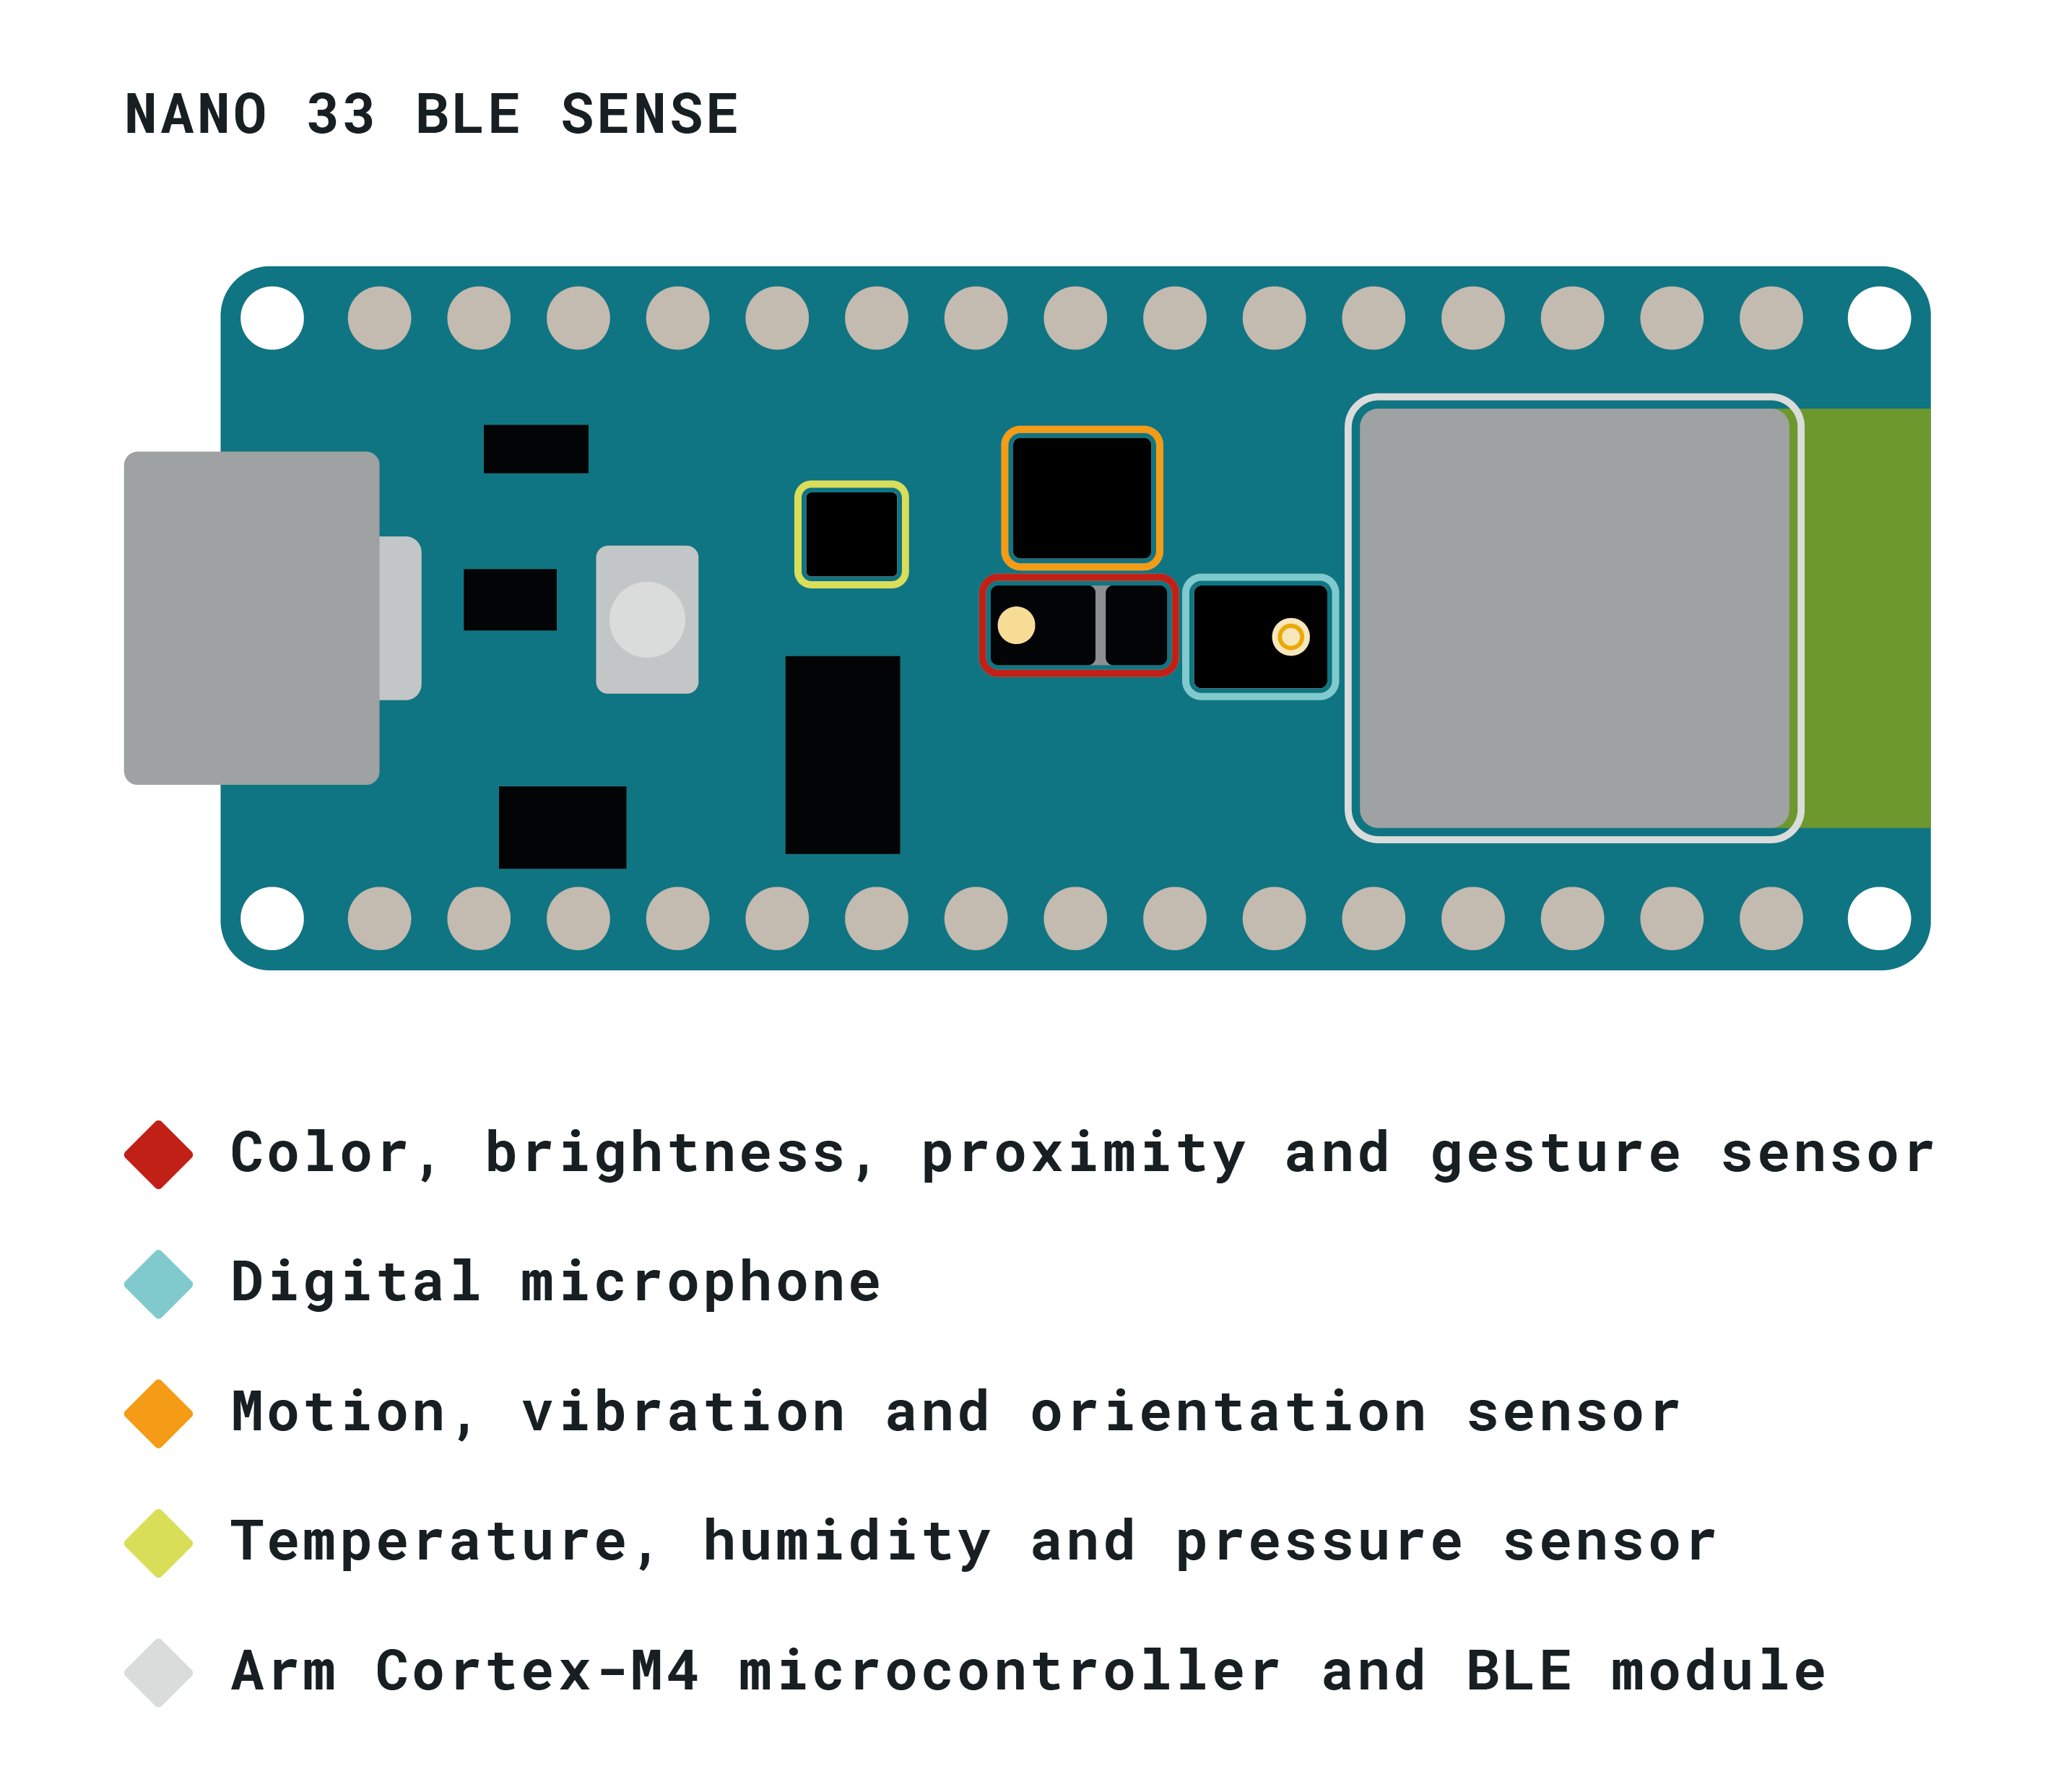
\includegraphics[width=0.5\linewidth]{Nano33BLESense/NANO-33-BLE-Sense_sensor-indentification}
	\caption{Arduino Nano 33 BLE Sense Sensors Placement} 
	\label{Arduino Nano 33 BLE Sense Architecture}
\end{figure}

The Arduino Nano 33 BLE Sense is an evolution of the traditional Arduino Nano, but featuring a lot more powerful processor, the nRF52840 from Nordic Semiconductors, a 32-bit ARM® Cortex™-M4 CPU running at 64 MHz.\cite{ArduinoNano33:2021} This will allow you to make larger programs than with the Arduino Uno (it has 1MB of program memory, 32 times bigger), and with a lot more variables (the RAM is 128 times bigger). The main processor includes other amazing features like Bluetooth® pairing via NFC and ultra low power consumption modes.

\section{Tiny-ML on Arduino Nano 33 BLE Sense}

Machine learning (ML) and Artificial intelligence (AI) are everywhere, its application, use cases and importance make it very usefull for every process. In the same sense, the tiny Arduino nano 33 BLE Sense board give us a way to make Tiny-ML application, where the model are not as big as previuosly made for high and big processing computer. By having a tiny machine learning model we can deploy it on low power devices, one of these is Arduino nano 33 BLE Sense. Due to its small size, the available set of sensors and low power consumption, it is easy to use anywhere by deploying the Machine leaarning algorithm and run the Internet of things (IOT) and Articial intelligence (AI) application for any process.\cite{Dokic:2020}

\section{Usefull Tiny-ML Model for Arduino Nano 33 BLE Sense}

\subsection{Voice Recognition}

Although, being a low power processing device it is not supported the big model and very big data. One of the usefull Tiny-ML model we can make on arduino nano 33 BLE Sense is to detect the different voices from the sorrounding. There is a on-board embed sensor on arduino for detecting voices is MP34DT05 the digital microphone. By using the MP34DT05, we can make a data set for keyword voice recognition model. Initially we train a model on Google colab and then convert it into TensorFlow lite for low power devices.\cite{Waqar:2021} For using the Voice recognition functionality of arduino nano 33 ble board, we need the on-board sensor MP34DT05 (Microphone), which is use for capturing, recognizing and detecting the voice. The supporting library for activating this sensor is PDM which will be discussed in the later chapter.

\subsection{Custom Gesture Recognition}

For capturing the gesture data using the on-board 9-axis Inertial measurement unit (IMU), we can make different types of gestures by rotating and changing the position by holding the arduino board in our hand . By doing this, the 9-axis IMU changes the accelerometre, and gyroscope value of the sensor. The limitation for training this model is to hold the board in our hand all the time. But, for the testing purpose it changes the valuse as per the gesture as shown in the figure below \ref{IMU Sensor Capture Data} for training the Tiny-Ml model.\cite{ArduinoNano33:2021}

\begin{figure}[ht]
	\centering
	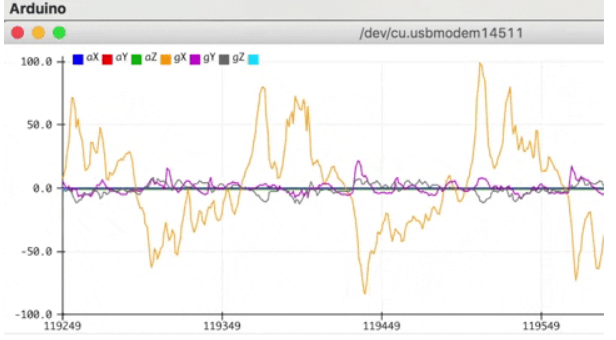
\includegraphics[width=0.5\linewidth]{Nano33BLESense/IMUData}
	\caption{IMU (Inertial Measurement Unit) Gesture Data} 
	\label{IMU Sensor Capture Data}
\end{figure}

The another possibility for detecting gesture is to use the APDS9960 sensor, it can also detect the gesture by moving the hand in front of it. It has also some limitation, it will not detect any gesture above 15 mm distance from the sensor.

\subsection{Color Detection}

The same above mentioned sensor APDS9960 is use for (Red, Green, Blue) RGB color detection too. We can also use the RGB functionality of this sensor and train the Tiny-ML model for detecting the different color product, which make the differentiation among the product on the basis of RGB color.

\subsection{Person Detection} 

One of the advantages of using a small devices such as the Arduino Nano 33 BLE Sense with TinyML is that it could be used as a remote low powered sensor to detect movement or even if there is a person in the area or not. APDS9960 sensor working as a proximity sensor, it can start to detect person at the certain distance. For doing this, we need external camera which can detect the moving person in the sorrounding or not. The supporting camera can be a Arducam Mini 2MP, which will be discuused in the hardware setup chapter later. Some usefull libraries e.g; JPEGDecoder library to decode JPEG-encoded images, the Arducam Library  need to be installed to make the compatibility between Arducam and edge computer (Arduino Nano 33 BLE Sense) by setting the hardware parametre in the library folder. The most necassary setting will be discussed in the later chapters too. \href{https://www.element14.com/community/community/project14/nano-rama/blog/2020/04/29/tinyml-on-arduino-nano-33-ble-sense-person-detection-with-ble}{Person Detection}

\section{General Overview Arduino Board}

Arduino consists of both a physical programmable circuit board (often referred to as a microcontroller) and a piece of software, or Integrated Development Environment (IDE) that runs on our computer, used to write and upload computer code to the physical board. Most of the arduino boards have both analog and digital General purpose input/output (GPIO) pins integrated on the board, depends upon the usage and functionality of the microcontroller embed on arduino board, these multipurpose GPIO makes it more usefull. By the advent of arduino, it make ease and get rid of external programming devices, we dont need to plug in and plug out our microcontrooler for programing the microcontroller. Arduino just need a connection with the computer with the help of USB, and we can upload the programm in a few second. \cite{Arduino:2021b}


